% Created 2018-06-05 Tue 08:50
% Intended LaTeX compiler: pdflatex
\documentclass[10pt]{beamer}
\usepackage[utf8]{inputenc}
\usepackage[T1]{fontenc}
\usepackage{graphicx}
\usepackage{grffile}
\usepackage{longtable}
\usepackage{wrapfig}
\usepackage{rotating}
\usepackage[normalem]{ulem}
\usepackage{amsmath}
\usepackage{textcomp}
\usepackage{amssymb}
\usepackage{capt-of}
\usepackage{hyperref}
\usetheme{Boadilla}
\author{ECON 499: Growth and Development}
\date{Spring 2018}
\title{Efficiency and Government}
\usecolortheme{seagull}
\usefonttheme[onlylarge]{structurebold}
\usefonttheme[onlymath]{serif}
\setbeamerfont*{frametitle}{size=\normalsize,series=\bfseries}
\setbeamertemplate{navigation symbols}{}
\setbeamertemplate{itemize item}[triangle]
\setbeamertemplate{footline}{}
\setbeamertemplate{enumerate items}[default]
\hypersetup{
 pdfauthor={ECON 499: Growth and Development},
 pdftitle={Efficiency and Government},
 pdfkeywords={},
 pdfsubject={},
 pdfcreator={Emacs 25.2.2 (Org mode 9.1.6)}, 
 pdflang={English}}
\begin{document}

\maketitle

\begin{frame}[label={sec:orgaa05141}]{}
\alert{Technology and growth}
\begin{itemize}
\item Solow model: long run growth (steady state) determined by growth rate in productivity
\item Endogenous growth: technology is \alert{created}, can be transferred across countries
\item Long-run growth rate of productivity the same across all countries
\end{itemize}
\end{frame}

\begin{frame}[label={sec:orgcbe65c3}]{}
\begin{center}
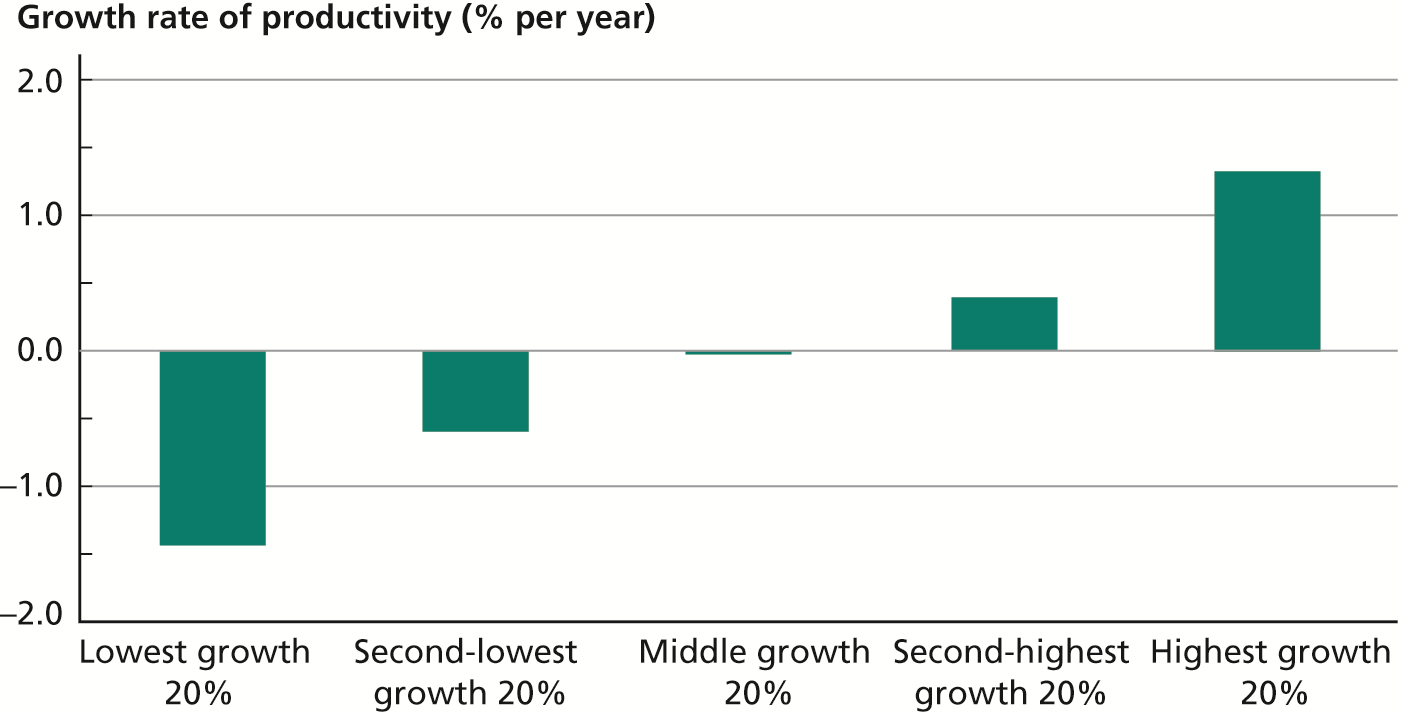
\includegraphics[width=.75\textwidth]{./img/7.6.png}
\end{center}
\end{frame}

\begin{frame}[label={sec:org78c8ec8}]{}
\alert{Efficiency and technology}
\begin{itemize}
\item Technology alone cannot account for cross-country differences in income/growth/productivity
\item Given a level of technology, countries likely differ in their ability to transform that tech into output (along with productive factors)
\item Some countries may be more \emph{efficient} than others
\end{itemize}
\end{frame}

\begin{frame}[label={sec:org53fa852}]{}
\alert{Pareto efficiency}
\begin{itemize}
\item Efficiency in economics usually refers to \emph{Pareto efficiency}
\item An allocation is Pareto efficient if no person can be made better off without making someone else worse off
\item All resources (factors) are being employed in their most effective way
\end{itemize}
\end{frame}

\begin{frame}[label={sec:orgcaa80e6}]{}
\alert{First fundamental theorem of welfare economics}
\begin{itemize}
\item In short: "market" allocations are Pareto efficient
\item Markets must be competitive and agents must be "well-behaved" (rational consumers, profit-maximizing firms)
\item Markets with incomplete information will not be Pareto efficient (Greenwald/Stiglitz, Akerlof, etc)
\end{itemize}
\end{frame}

\begin{frame}[label={sec:org2400c9d}]{}
\alert{ECON 311}
\begin{itemize}
\item Profit maximizing firms employ factors until the value of the marginal product is equal to factor compensation
\item \(pMPL = w\)
\item In competitive markets, everyone who wants to work at the market wage can find a job, everyone who wants to employ a worker at the market wage can find an employee (supply=demand)
\end{itemize}
\end{frame}

\begin{frame}[label={sec:org1410c15}]{}
\alert{5 types of inefficiency}
\begin{enumerate}
\item Unproductive activities
\item Idle resources
\item Factor misallocation
\item Misallocation among firms
\item Technology blocking
\end{enumerate}
\end{frame}

\begin{frame}[label={sec:org9f072e7}]{}
\alert{1. Unproductive activities}
\begin{itemize}
\item Theft and other crime is "unproductive," people spend resources to protect themselves that could be spent elsewhere
\item Example: Average Russian retail firm pays 20\% of revenue for "protection"
\item Using the government to protect unproductive work is called \emph{rent seeking}
\item Examples: Licenses, monopolies, import quotas, tariffs, etc
\end{itemize}
\end{frame}

\begin{frame}[label={sec:org0506790}]{}
\alert{2. Idle resources}
\begin{itemize}
\item Factors that are not utilized or underutilized are considered idle (unemployed workers, unused factories, etc)
\item Large bureaucratic institutions often have underemployed resources, hire more than is necessary
\item Agriculture subsidies in US -- landowners paid to \emph{not} grow crops
\end{itemize}
\end{frame}

\begin{frame}[label={sec:org799aeeb}]{}
\alert{3. Misallocation among sectors}
\begin{itemize}
\item Workers and resources can be misallocated between industries
\item Competitive markets: \(w = pMPL\)
\item Higher wages should attract workers, eliminating differences
\item Some \emph{friction} is required to keep markets from allocating efficiently across sectors
\end{itemize}
\end{frame}

\begin{frame}[label={sec:orgd4a2702}]{}
\alert{Frictions}
\begin{itemize}
\item Mobility
\begin{itemize}
\item Workers may not move to new sector because of geography, laws, culture, etc
\item Minimum wages in certain regions/sectors can prevent firms from hiring lower-wage workers
\end{itemize}
\item Wages and MPL
\begin{itemize}
\item Some firms may allocate surplus evenly across workers (co-ops, family farms, etc). These workers are earning pAPL, not pMPL
\item Discrimination may prevent employers from hiring otherwise qualified applicants
\end{itemize}
\end{itemize}
\end{frame}

\begin{frame}[label={sec:org2068f60}]{}
\alert{4. Misallocation among firms}
\begin{itemize}
\item Firms within industries have different productivities
\item Governments may subsidize certain firms, exempt from regulation
\item Within-industry productivities vary more in developing countries
\end{itemize}
\end{frame}

\begin{frame}[label={sec:orgbaf0b93}]{}
\alert{5. Technology blocking}
\begin{itemize}
\item Technological improvements often disadvantage some workers
\item These workers can use political power to stop technology from being implemented
\item Examples: Printing press, Luddites, railroads, AC electricity, margarine, AI, pharmaceuticals
\item For many, it is rational to oppose technological change despite impact on growth
\end{itemize}
\end{frame}

\begin{frame}[label={sec:orge1cd1bf}]{}
\alert{Central planning in the USSR}
\begin{itemize}
\item Higher factor accumulation than US, similar technology
\item GDP per capita was 1/3 of US in 1985
\item Labor, capital, raw materials allocated by government bureaucrats rather than market
\item Different incentives for workers -- managers trying to meet quotas (not maximizing profits), workers paid regardless of effort
\end{itemize}
\end{frame}

\begin{frame}[label={sec:orgf51b8f4}]{}
\alert{Hayek's local information}
\begin{itemize}
\item Friedrich Hayek: \emph{local information} makes planning ineffective
\end{itemize}
\begin{quote}
"To know of and put to use a machine not fully employed, or somebody's skill which could be better utilized, or to be aware of a surplus stock which can be drawn upon during an interruption of supplies, is socially quite as useful as the knowledge of better alternative techniques. And the shipper who earns his living from using otherwise empty or half-filled journeys of tramp-steamers, or the estate agent whose whole knowledge is almost exclusively one of temporary opportunities, or the arbitrageur who gains from local differences of commodity prices, are all performing eminently useful functions based on special knowledge of circumstances of the fleeting moment not known to others."
\end{quote}
\end{frame}

\begin{frame}[label={sec:org06130ec}]{}
\alert{Chinese economic reform}
\begin{itemize}
\item Command economy after the civil war (1950)
\item Collective agriculture, no foreign investment, public ownership of firms
\item Low growth, poor distribution of resources (frequent famines)
\item Deng Xiaoping reforms in 1978: private control over farm plots, state-owned enterprises allowed to sell excess production in markets
\item 1980s: Increased privatization, opened credit markets
\item Rapid growth followed from reforsm
\end{itemize}
\end{frame}

\begin{frame}[label={sec:org8b6291b}]{}
\alert{Finance}
\begin{itemize}
\item Robust financial sector is highly correlated with growth
\item Investors seek to maximize returns
\item Returns on investment are the productivity of capital (\(r=MPK\))
\item Financial system allocates capital to most productive processes
\item Financial system can also allocate \emph{risk} efficiently (in theory\ldots{})
\end{itemize}
\end{frame}

\begin{frame}[label={sec:org6bd62b7}]{}
\alert{Proximate causes of growth}
\begin{itemize}
\item Factor accumulation
\item Human capital
\item Efficiency
\item Technology
\item Trade openness
\end{itemize}
\end{frame}

\begin{frame}[label={sec:orgfc2380e}]{}
\alert{Fundamental causes}
\begin{itemize}
\item Why do some countries accumulate capital? Why do some have higher technology? Efficiency? etc
\item What explains differences in proximate causes?
\item Government/institutions, culture, geography, natural resources\ldots{}
\end{itemize}
\end{frame}

\begin{frame}[label={sec:org0cd462c}]{}
\alert{Market failures}
\begin{itemize}
\item Public goods
\item Externalities
\item Monopoly
\item Coordination failure
\item Distributional concerns
\end{itemize}
\end{frame}

\begin{frame}[label={sec:orgc0a1ff2}]{}
\alert{Government failures}
\begin{itemize}
\item Inefficient factor employment (post office, DMV, etc)
\item Deregulation often results in lower prices, more access (airlines, telecoms)
\item Equity/efficiency trade-off?
\end{itemize}
\end{frame}

\begin{frame}[label={sec:org6a3aad0}]{}
\alert{Government and growth}
\begin{itemize}
\item How do government policies impact growth? Four dimensions:
\begin{enumerate}
\item Rule of law
\item Size of government
\item Planning/nationalization
\item Civil conflict
\end{enumerate}
\end{itemize}
\end{frame}

\begin{frame}[label={sec:orgc06a5b8}]{}
\alert{Rule of law}
\begin{itemize}
\item Firms enter into contractual agreements
\item Government enforces contracts
\item Courts and bureaucracy respond to rules or politics?
\item Investment risky when contracts not enforced
\end{itemize}
\end{frame}

\begin{frame}[label={sec:org0af4b91}]{}
\begin{center}
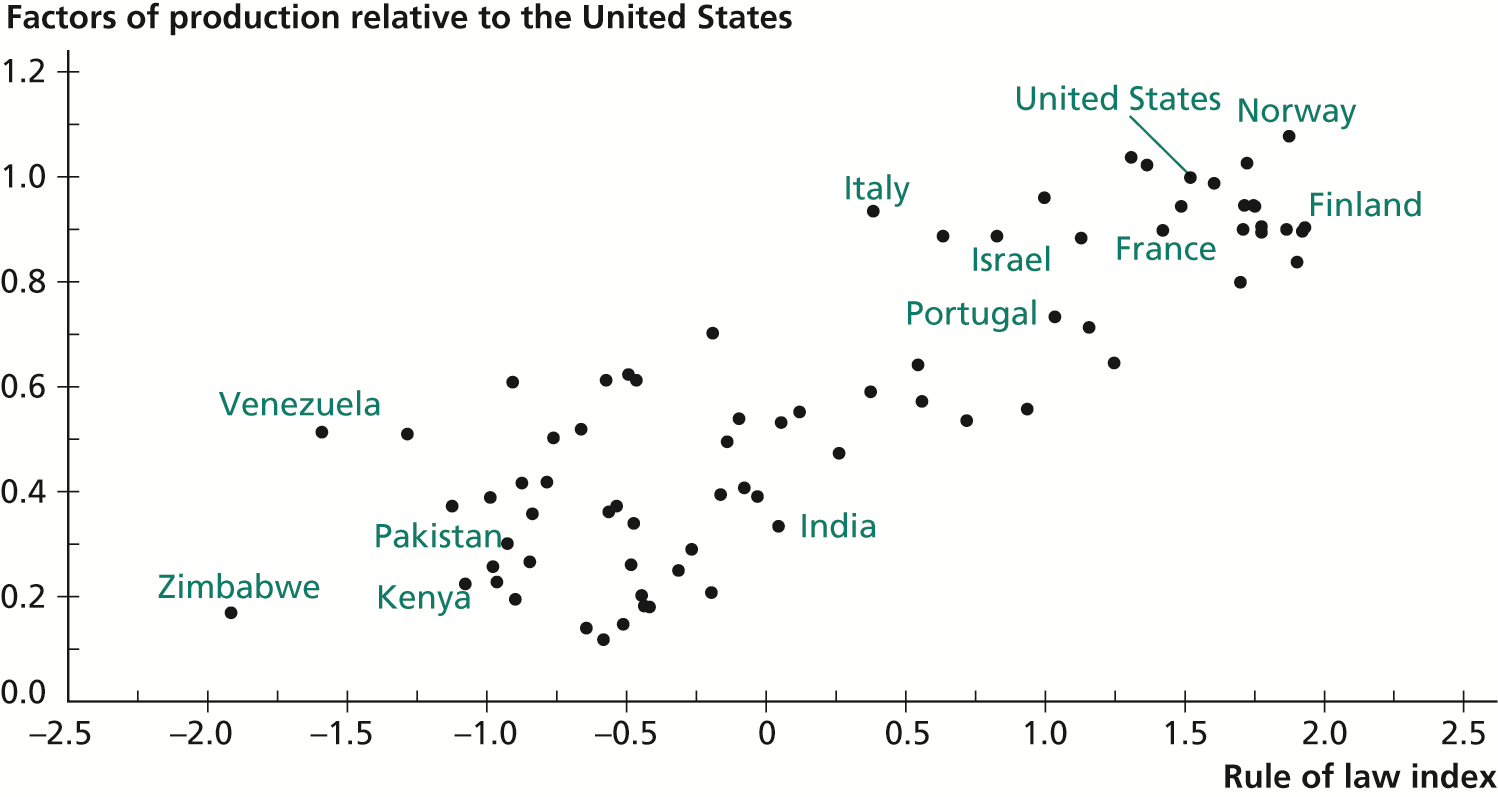
\includegraphics[width=.75\textwidth]{./img/12.1.png}
\end{center}
\end{frame}

\begin{frame}[label={sec:org7139d94}]{}
\begin{center}
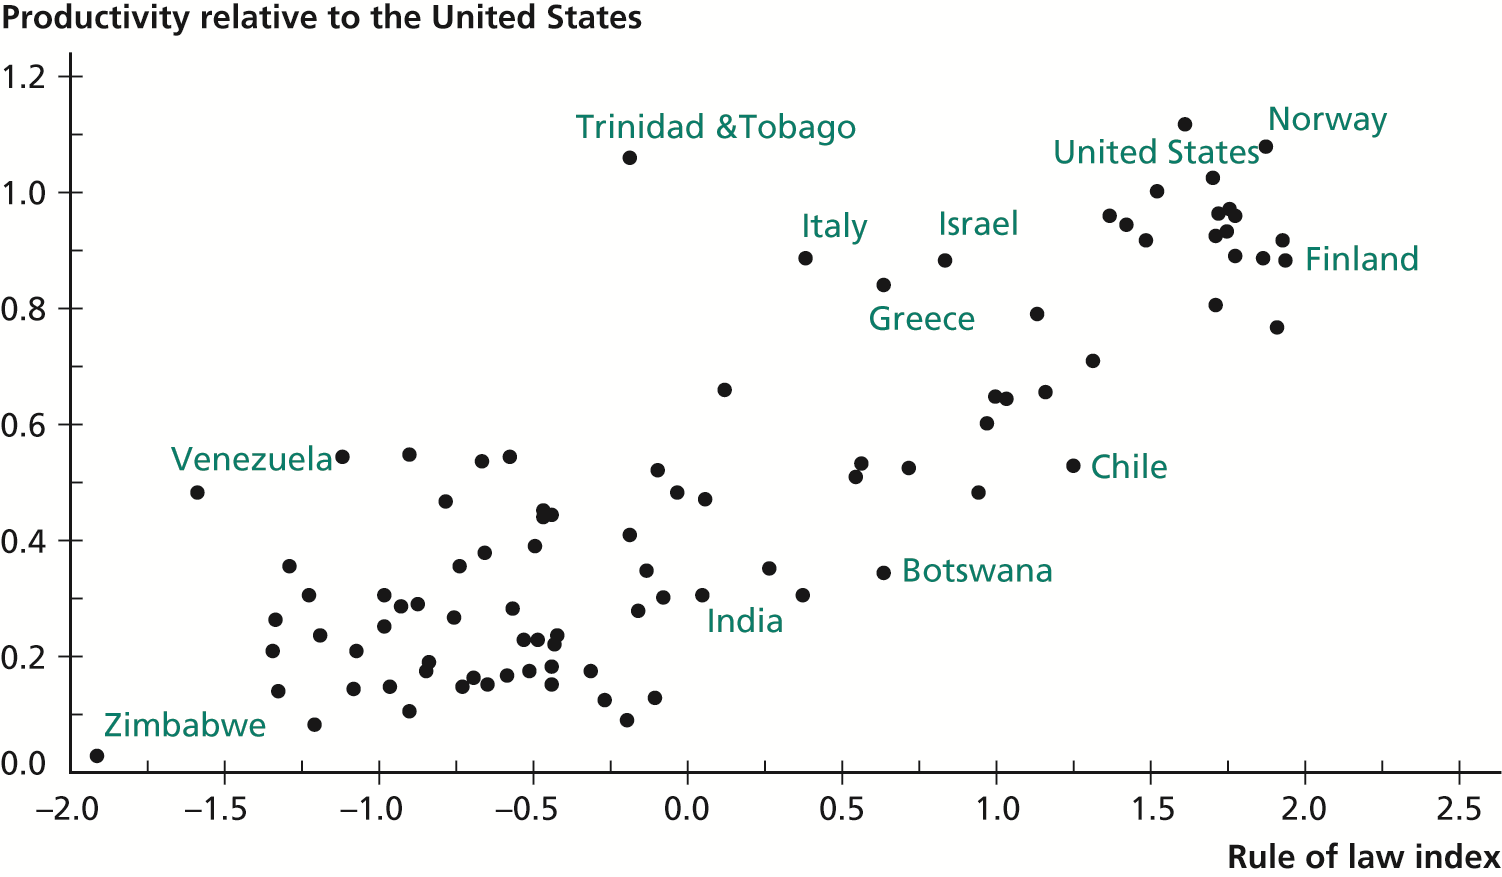
\includegraphics[width=.75\textwidth]{./img/12.2.png}
\end{center}
\end{frame}

\begin{frame}[label={sec:org01685ca}]{}
\alert{Size of government}
\begin{itemize}
\item Governments that spend must also raise revenue (tax)
\item Taxation is often inefficient (ECON201)
\item Wagner's law: Developed economies more complex, need larger government to enforce complex rules
\item Trade-off between rule of law enforcement and tax DWL
\end{itemize}
\end{frame}

\begin{frame}[label={sec:org5bd1ee1}]{}
\alert{Planning}
\begin{itemize}
\item State enterprises often are not maximizing profits \(\rightarrow\) inefficient
\item Costs usually fall after privatization
\end{itemize}
Benefits of planning:
\begin{itemize}
\item "Infant industries:" Korean steel and chemicals
\item Technology: Taiwan allowed FDI only if firms transfer tech to local firms
\item Korean and Taiwanese firms quickly privatized once competitive internationally
\end{itemize}
\end{frame}

\begin{frame}[label={sec:org36f970f}]{}
\alert{Civil conflict}
\begin{itemize}
\item Wars and conflict destroy factors, infrastructure, human capital acquisition
\item Poverty and crime have similar effects
\item Strong governments can prevent conflict, encouraging growth
\item "Conflict trap:" Low growth \(\rightarrow\) conflict \(\rightarrow\) low growth
\end{itemize}
\end{frame}

\begin{frame}[label={sec:org6767351}]{}
\alert{Extractive institutions}
\begin{itemize}
\item Some governments enact policy that benefits government officials and their associates
\item Taxation and policy transfer wealth from workers to government officials
\item Policies that create opportunity for bribery
\item Self preservation: growth increases education and awareness, may hasten political reform
\end{itemize}
\end{frame}

\begin{frame}[label={sec:org14b15ba}]{}
\begin{center}
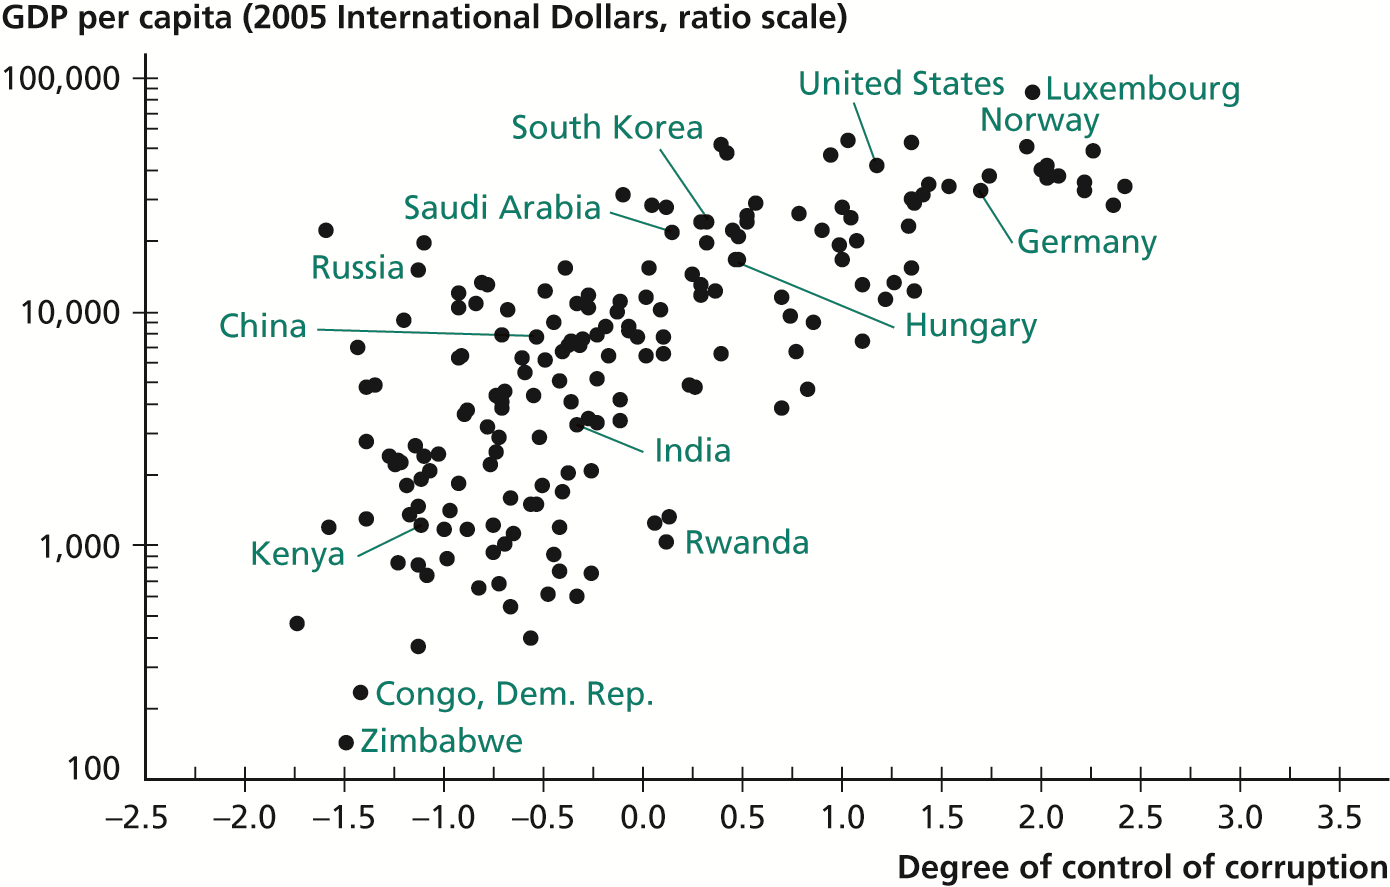
\includegraphics[width=.75\textwidth]{./img/12.5.png}
\end{center}
\end{frame}

\begin{frame}[label={sec:org06f1358}]{}
\alert{Causation}
\begin{itemize}
\item Government institutions and growth are correlated
\begin{itemize}
\item Growth causes government?
\item Government causes growth?
\item Cause each other?
\item Third factor causes both?
\item Instruments?
\end{itemize}
\end{itemize}
\end{frame}

\begin{frame}[label={sec:orge1992a9}]{}
\alert{Acemoglu, Johnson, Robinson (2001)}
\begin{itemize}
\item \emph{Colonial Origins of Comparative Development}
\item Use early settler mortality as an instrument for current governmental institutions
\item Settler mortality \(\rightarrow\) early institutions \(\rightarrow\) modern institutions
\item Results: Government has substantial impact on growth
\end{itemize}
\end{frame}

\begin{frame}[label={sec:org7371054}]{}
\alert{Inequality}
\begin{itemize}
\item Equity/efficiency trade-off?
\item Does redistribution decrease growth?
\item Gini coefficient:
\begin{itemize}
\item \(=0\) if no inequality
\item \(=1\) if "perfect" inequality
\end{itemize}
\end{itemize}
\end{frame}

\begin{frame}[label={sec:org3cd4f61}]{}
\alert{Kuznets hypothesis}
\begin{itemize}
\item "Inverted-U"
\item Low income, agricultural societies have low inequality
\item Urban areas develop, urban incomes diverge
\item Labor mobility decreases inequality as country develops
\end{itemize}
\end{frame}

\begin{frame}[label={sec:org0e0ce12}]{}
\begin{center}
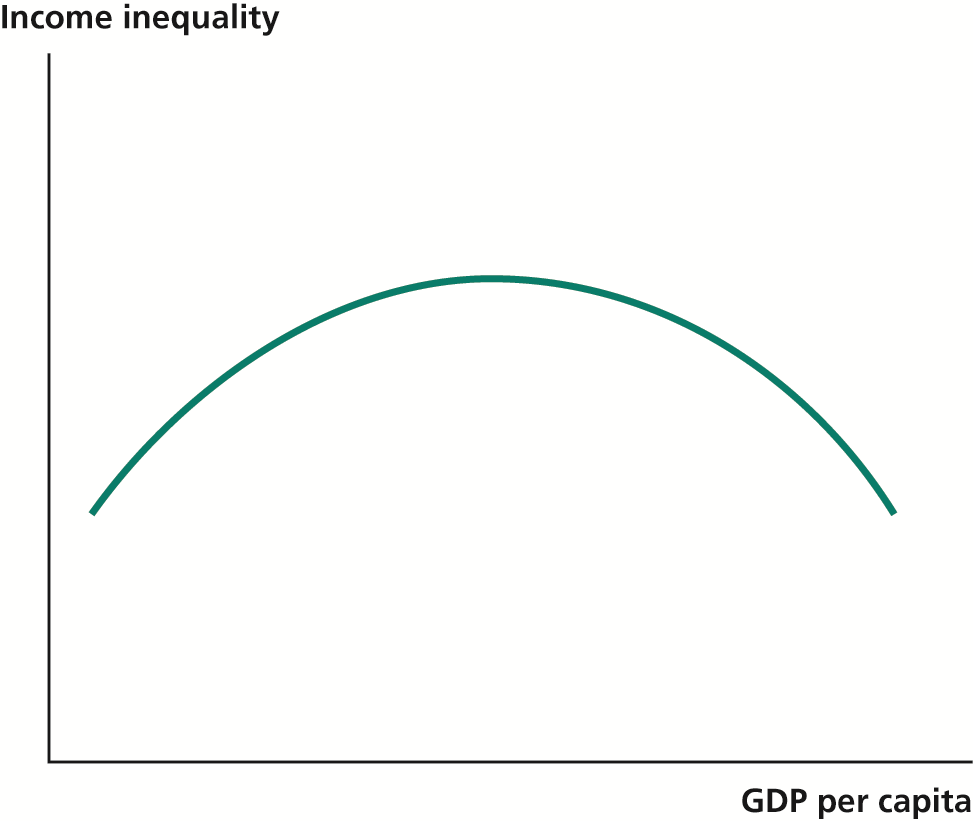
\includegraphics[width=.75\textwidth]{./img/13.3.png}
\end{center}
\end{frame}

\begin{frame}[label={sec:org55280e3}]{}
\begin{center}
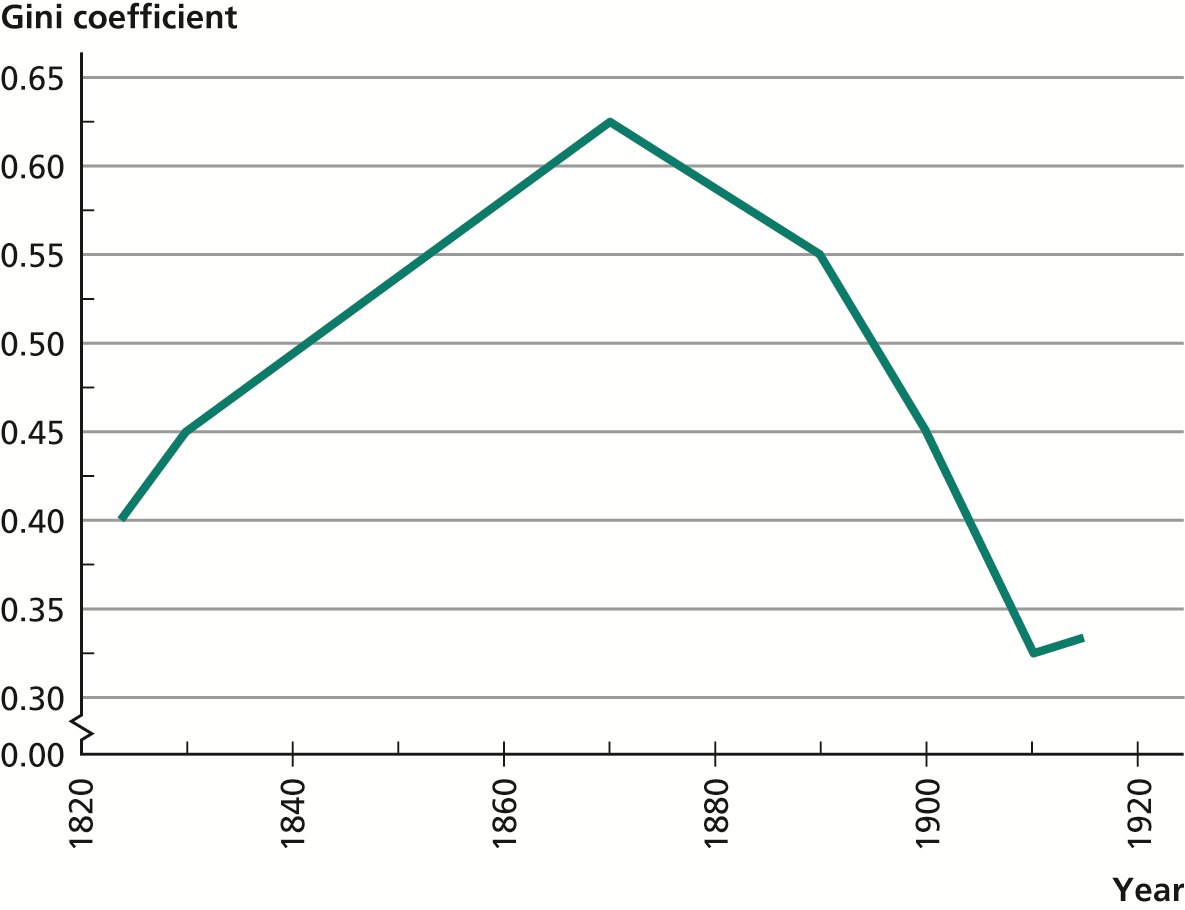
\includegraphics[width=.75\textwidth]{./img/13.4.png}
\end{center}
\end{frame}

\begin{frame}[label={sec:orgbbd435c}]{}
\begin{center}
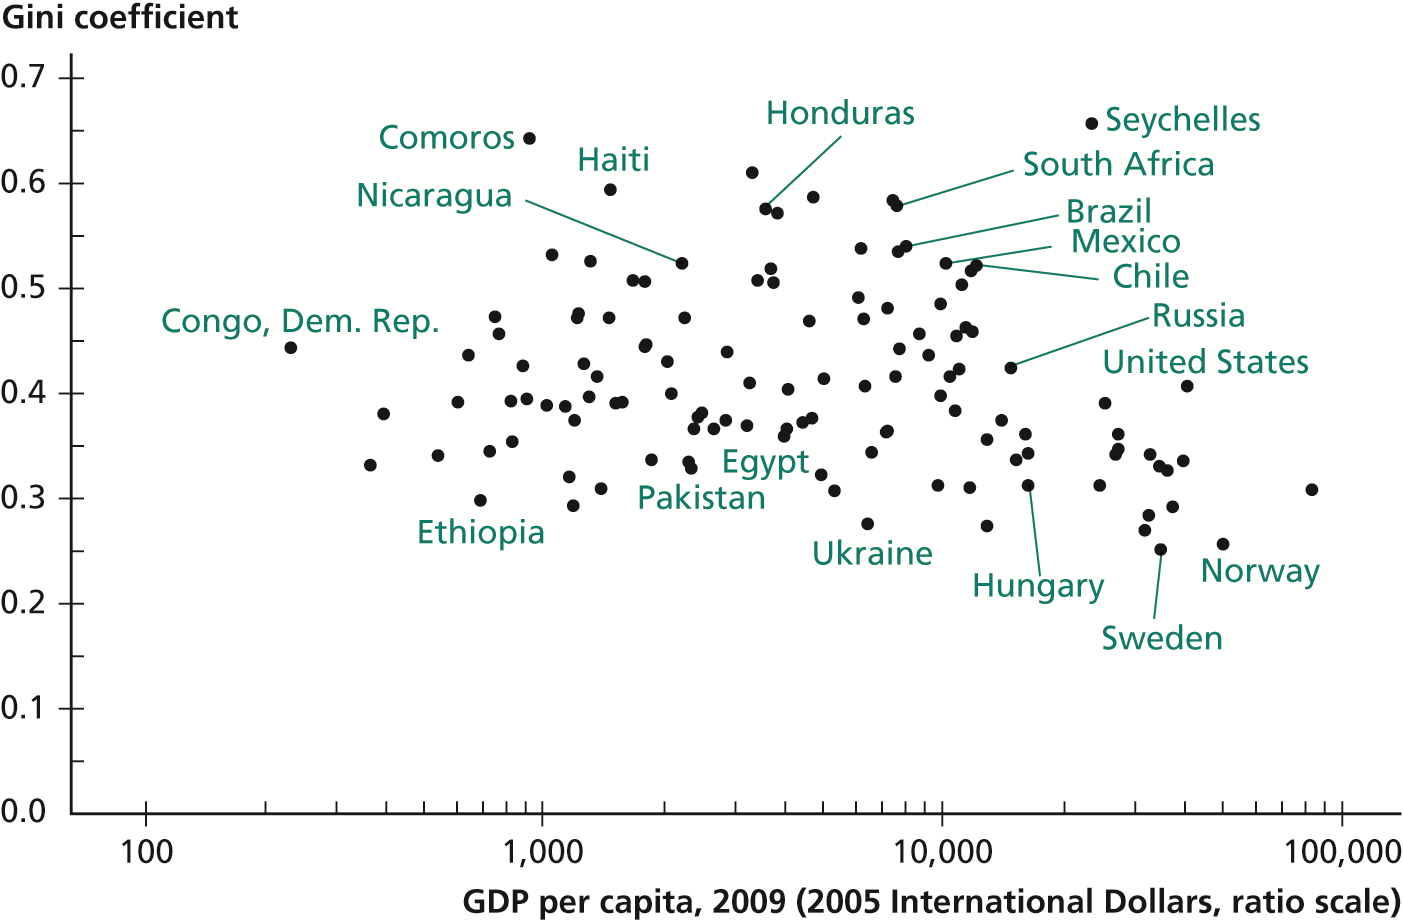
\includegraphics[width=.75\textwidth]{./img/13.5.png}
\end{center}
\end{frame}

\begin{frame}[label={sec:orgb36208f}]{}
\alert{Inequality and physical capital}
\begin{itemize}
\item More inequality \(\rightarrow\) more income in hands of the rich
\item Rich save a higher percentage of income than poor
\item Average savings rate \((\gamma )\) increases, higher SS
\end{itemize}
\end{frame}

\begin{frame}[label={sec:org1e5e3a5}]{Human capital and physical capital}
\begin{center}
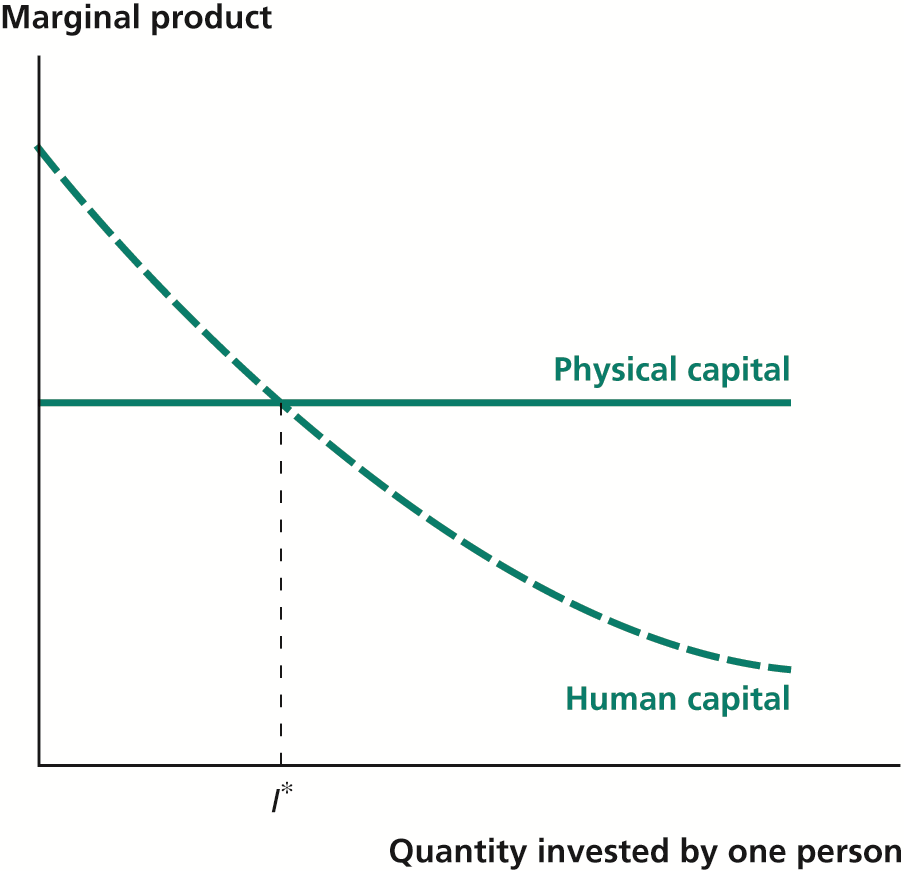
\includegraphics[width=.75\textwidth]{./img/13.11.png}
\end{center}
\end{frame}

\begin{frame}[label={sec:orgf40697c}]{}
\alert{Redistribution and growth}
\begin{itemize}
\item Second fundamental theorem of welfare economics: "Lump sum" transfers are efficient
\item Rich may hide assets, cheat to avoid taxes
\item Unrest: high inequality may cause political unrest, crime
\item Reducing inequality can alleviate social pressures that are bad for growth
\item Causality?
\end{itemize}
\end{frame}

\begin{frame}[label={sec:org4c1370d}]{}
\alert{Empirical evidence}
\begin{itemize}
\item Lower human capital in places with inequality
\item Inequality does not appear to be related to unrest
\item Inequality does not cause more redistribution
\end{itemize}
\end{frame}
\end{document}